\documentclass{homework}
% \usepackage{graphicx} % Required for inserting images
\usepackage{amsmath}
\usepackage{gensymb}
\usepackage{subfig}
\usepackage{float}
\usepackage[framed,numbered,autolinebreaks,useliterate]{mcode}

\class{ECEN 5244}
\title{Homework 4}
\author{Sean Jennings}
\date{October 2, 2024}

\begin{document}
\maketitle

\section{Problem 1}
\begin{letterenum}
\item Periodogram
\begin{enumerate}[label=\roman*)]
\item The overlayed spectrum computed using the various window
function  are shown in Figures \ref{fig:various-windows} and
\ref{fig:various-windows-zoom}.

\begin{center}
    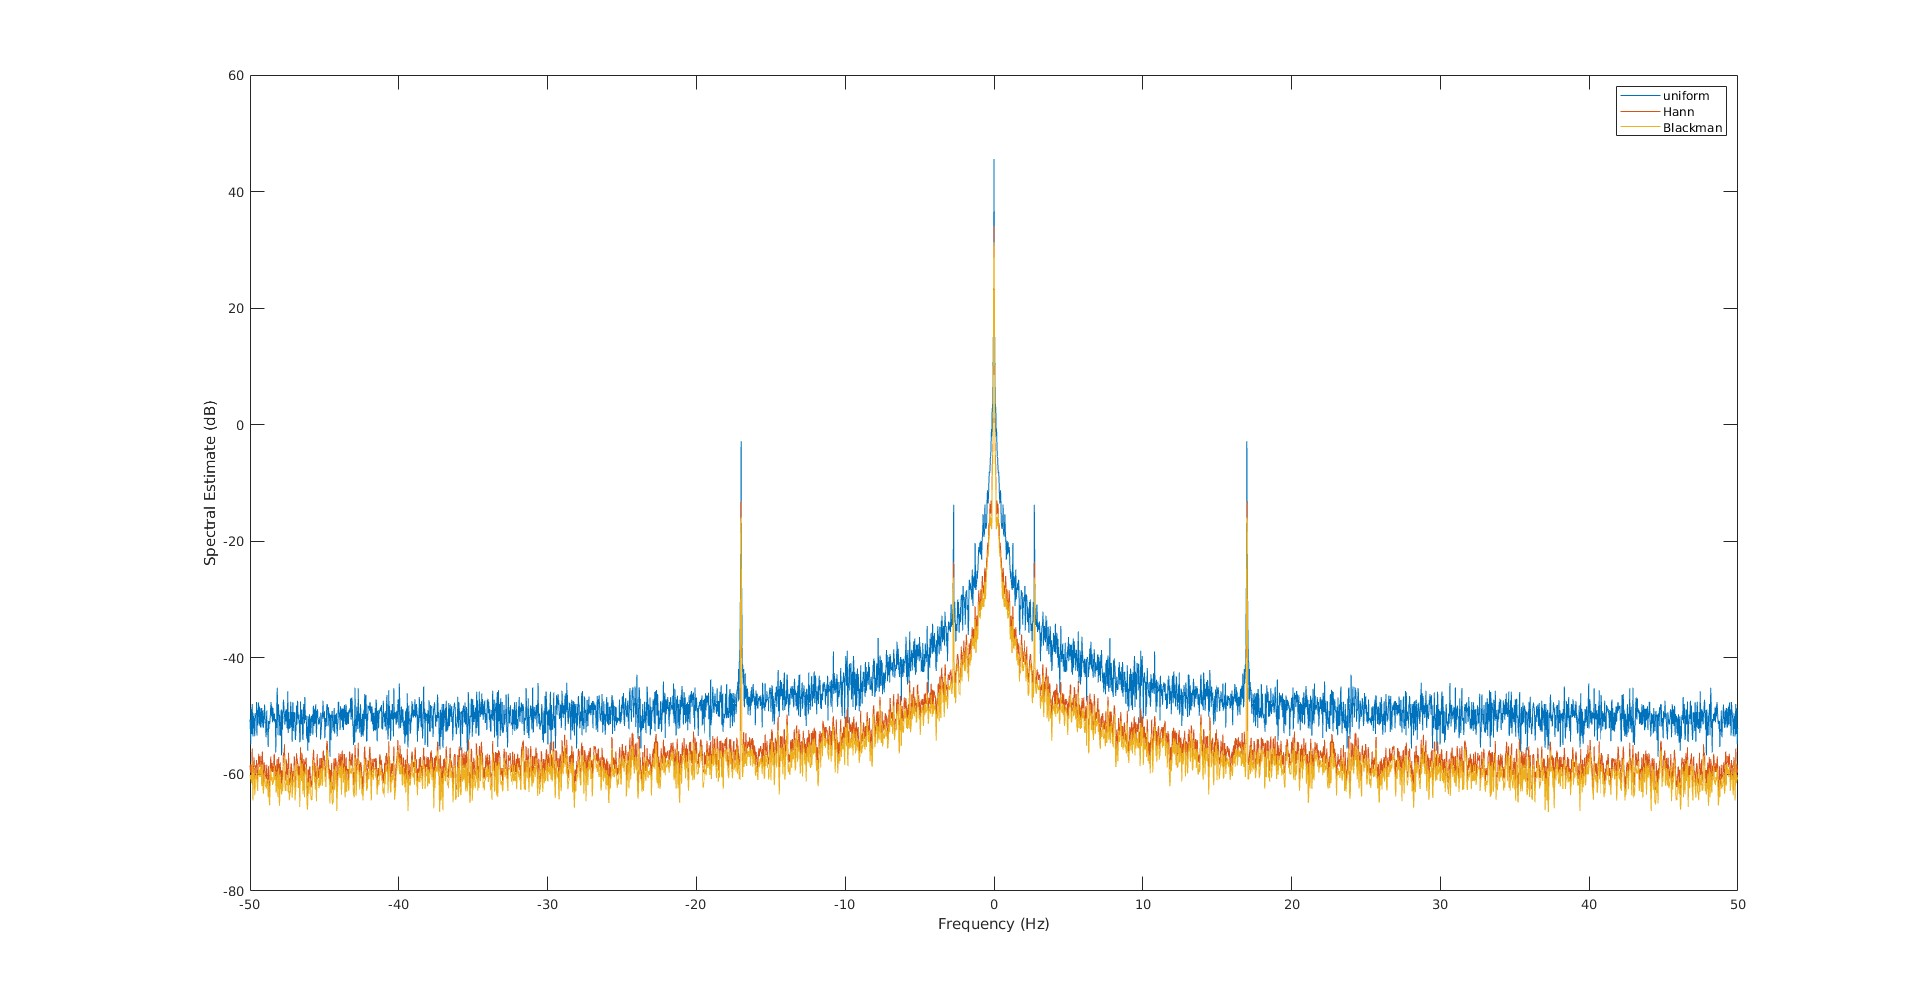
\includegraphics[width=\linewidth]{Images/across_windows.jpg}
    \captionof{figure}{
        Spectral Power Density computed via Periodogram using
        variety of windowing functions}
    \label{fig:various-windows}
\end{center}

\begin{center}
    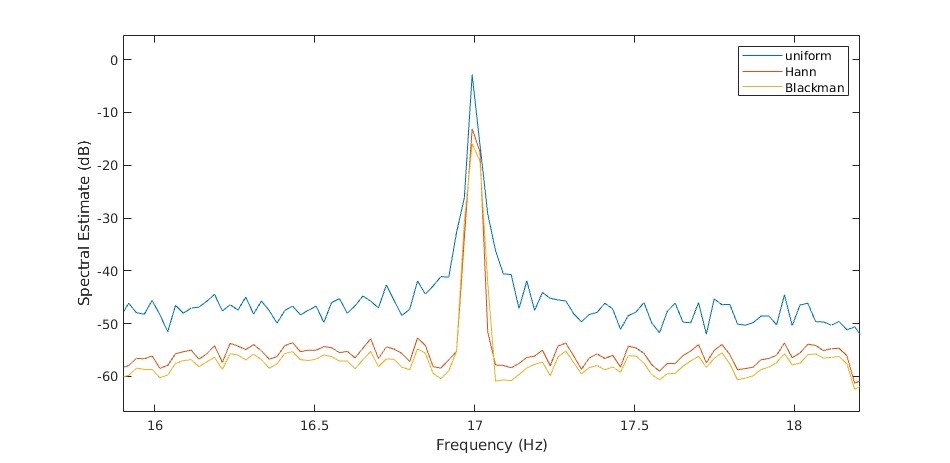
\includegraphics[width=\linewidth]{Images/across_windows_zoom.jpg}
    \captionof{figure}{Zoomed on 17 Hz peak}
    \label{fig:various-windows-zoom}
\end{center}

\item
\item
\item The spectral resolution is:
\begin{equation*}
    \Delta f = \frac{1}{N\Delta} = 0.0244 \text{ Hz}
\end{equation*}
where $\Delta = 0.01$ seconds is the time between samples and $N=4096$ is the number
of samples used to compute the DFT.

\item The spectral resolution is related to $N$ which is held constant
for each window and is therefore equal for each windowing function. The uniform
window has the narrowest at the peak, reflecting the fact that the main lobe of
the uniform window is narrower compared to the Hann and Blackman window functions.
However, there is a wider frequency range over which the uniform windowed estimate
remains above noise levels. This reflects greater spectral leakage into the side lobes.

The Hann and Blackman windows are quite similar to each other. The top of the peak
is wider than the uniform window, but the total width of frequencies which are
above noise levels is smaller compared to the uniform window.

Across frequencies, the magnitude of the uniform windowed estimate is greater than
the Hann estimate, which in turn is (slightly) greater than the Blackman estimate.
This reflects the fact that multiplication of the signal by the windowing function
reduces the power in the spectral estimate.

\item Figures \ref{fig:various-windows-lengths} and \ref{fig:various-windows-lengths-zoom}
show the Periodogram-estimated spectral density with the length of the window
varied.

\begin{center}
    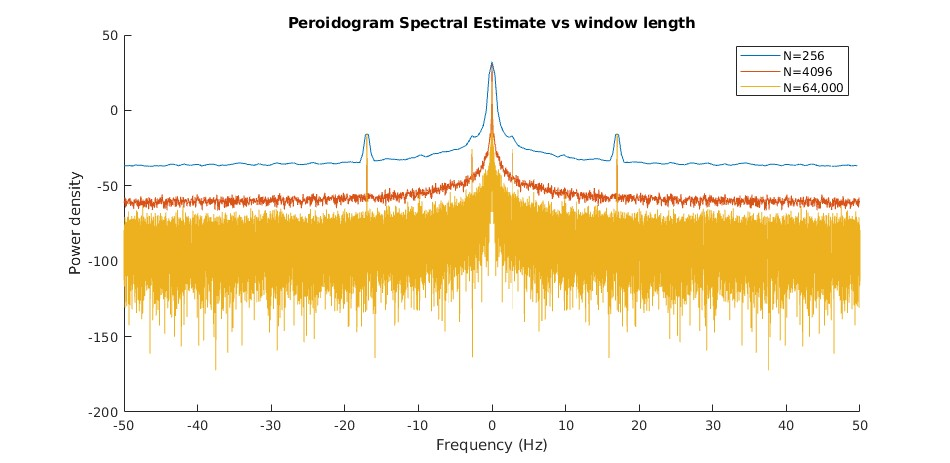
\includegraphics[width=\linewidth]{Images/across_window_length.jpg}
    \captionof{figure}{Spectral Estimates for Different Window Lengths}
    \label{fig:various-windows-lengths}
\end{center}
\begin{center}
    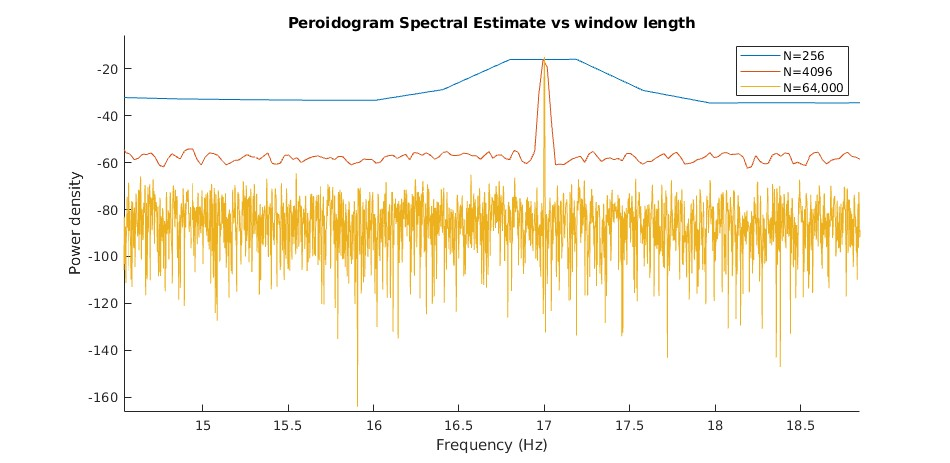
\includegraphics[width=\linewidth]{Images/across_window_length_zoom.jpg}
    \captionof{figure}{Zoomed on 17 Hz Peak}
    \label{fig:various-windows-lengths-zoom}
\end{center}

\item The amount of spectral leakage into the side-lobes is significantly higher
for the estimates that are generated with shorter window lengths. The width
of the side lobes is a function of the frequency resolution $\Delta f$, so 
the increased resolution with higher window legnths means that the spectral
leakage decays faster.

\end{enumerate}

\item
\begin{enumerate}[label=\roman*)]
\item The autocorrelation function is shown in Figure \ref{fig:autocorrelation}.

\begin{center}
    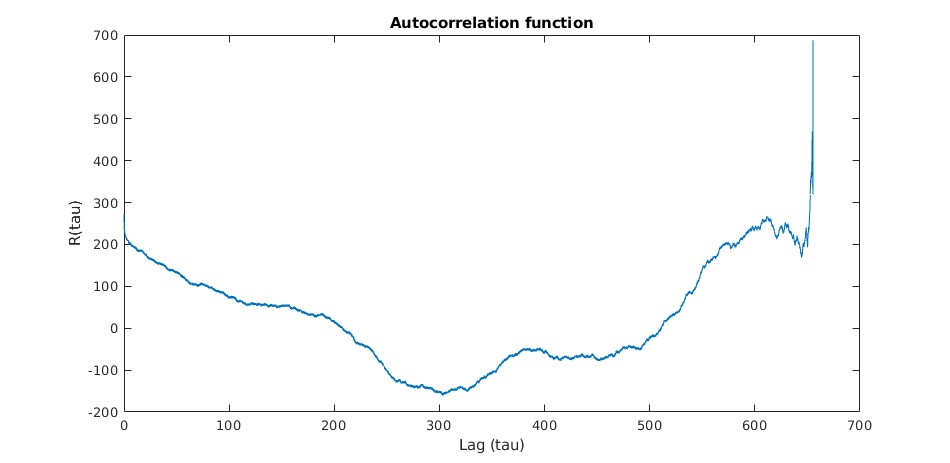
\includegraphics[width=\linewidth]{Images/autocorrelation.jpg}
    \captionof{figure}{Autocorrelation function}
    \label{fig:autocorrelation}
\end{center}

\item The autocorrelation function increases dramatically for high values
of lag. This is because the autocorrelation function evaluated at $\tau = n\Delta$
(some integer multiple of the sample time) estimates the expectation
$E{x_t x_{t - \tau}}$ by taking the average over $L-n$ samples (where $L$ is the
total number of samples in the full signal). Thus, large lags are averaged over
less samples, resulting in a greater variance.

Using these high lag values in our spectral estimate will introduce noise to the
estimate.

\item Since the autocorrelation function is given by:
\begin{equation*}
    R(\tau) = \lim_{T\to\infty} \frac{1}{2T} \int_{-T}^{T} x(t + \tau) x^*(t) dt
\end{equation*}
which can be approximated by
\begin{equation*}
    R_n = \frac{1}{L-n} \sum_{i=1}^{L-n} x_i x_{i+n}^*
\end{equation*}
The total power in the signal is given by:
\begin{equation*}
    R_0 = \frac{1}{L} = \sum_{i=1}^L |x_i|^2
\end{equation*}
So, the power is simply given by the first entry of the assymetric autocorrelation
function. This computation in MATLAB yields: 270.605.

\item Figures \ref{fig:BT-method} and \ref{fig:BT-method-zoom} show the Blackman-Tukey
estimate for the desired lag indices.

\begin{center}
    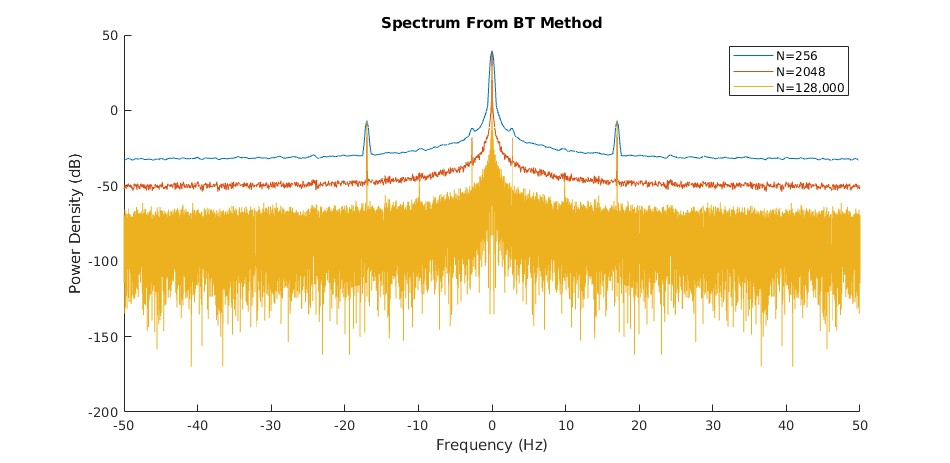
\includegraphics[width=\linewidth]{Images/BT_method.jpg}
    \captionof{figure}{Spectral Estimate from Blackman-Tukey Method}
    \label{fig:BT-method}
\end{center}

\begin{center}
    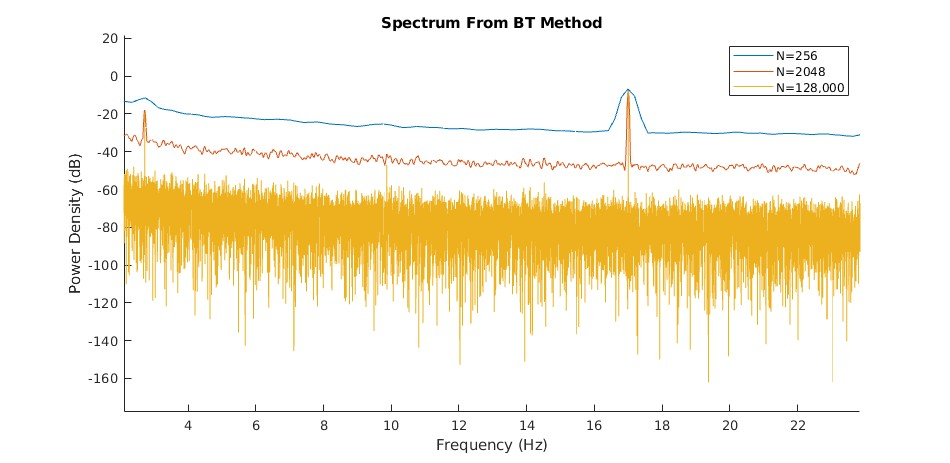
\includegraphics[width=\linewidth]{Images/BT_method_zoom.jpg}
    \captionof{figure}{Zoomed BT estimate}
    \label{fig:BT-method-zoom}
\end{center}

\item The power can be estimated from the spectral power density by simply
summing over all frequencies:
\begin{equation*}
    \sum_{k=-2N}^{N} S(f_k)
\end{equation*}
However, because we perform a normalization step in the code
(per the "Normalization of $S_x(f_k)$" lecture slide), this gives
an identical result to part iii).

\end{enumerate}
\end{letterenum}

\section{Problem 2}
\begin{letterenum}
\item The variance in the voltage signal $\sigma_V^2$ is the RMS of the signal
and is given by:
\begin{equation*}
    \sigma_V^2 = |V_{RMS}|^2 = P R = (10 \text{ mW}) \cdot (50 \ohm) = 5e^{-2} \text( V^2)
\end{equation*}
The variance in noise $\sigma_{V_c}$ is related to the discrezation step $\Delta V$
by:
\begin{equation*}
    \sigma_{V_c} = \frac{\Delta V}{\sqrt{12}} = \frac{V_{max} - V_{min}}{\sqrt{12} \cdot 2^{N_b}}
\end{equation*}
where $N_b = 12$ is the number of bits.

We want the variance in noise to be 1\% of the variance in the signal voltage, so
\begin{equation*}
    \sigma_{V_c}^2 \leq 0.01 \sigma_V^2 = 5e^{-4}
\end{equation*}
Combining these equations, we have the range of the ADC converter must be no more than:
\begin{equation*}
    V_{max} - V_{min} = \Delta V \cdot 2^{N_b} = \sqrt{12} \cdot \sigma_{V_c} \cdot 2^{N_b}
        \leq \sqrt{12} \cdot \sqrt{5e{-4}} \cdot 2^{12} = 317.27 \text{ (V)}
\end{equation*}
for the variance in discretization noise to be less than 1\% of the signal noise.

\item One possible situation which would cause the discretization noise to not be
white is if there were nonlinearities in the ADC which were not properly accounted for.
Such a nonlinearity could cause the width of the discretization to be $\Delta V$ to
not be constant across the range of the device. Then, if a periodic input signal
had a peak-to-peak range which spanned across two effective discretization widths 
$\Delta V_1$ and $\Delta V_2$, the noise would be greater in one portion of the
input's period than the other. The spectrum of the noise would then have increased
power density around harmonics of the input signal, making it no longer "white".
    
\end{letterenum}

\section{Appendix: Code}
\begin{lstlisting}
load hw4.mat d

function w = uniform_window(m)
    w = ones(m, 1);
end

function w = hann_window(n)
    w = 0.5 * (1 - cos(2 * pi * (0:n-1)' / (n-1)));
end

function w = blackman_window(n)
    % Use 0:m-1 so that the window has size m and is symmetric starting
    % and ending at 0.
    x = (0:n-1)' / (n-1);
    w = 0.42 - 0.5 * cos(2 * pi * x) + 0.08 * cos(4 * pi * x);
end

function S = periodogram(x, N, overlap, window_func)
    L = size(x, 1);  % Total number of samples
    M = floor((L-overlap) / (N - overlap));

    w = window_func(N);
    S = zeros(N,1);
    index = 1:N;
    for i=1:M
        S = S + abs(fft(x(index) .* w)).^2;
        index = index + (N - overlap);
    end
    S = fftshift(S) / (M * N^2);
end


x = d(:, 1); y = d(:, 2);

% Part A i)-iii) Varying window functions
N = 4096;
overlap = N / 4;
t = d(:, 1); x = d(:, 2);
figure()
plot(t, x)
title("Signal")
xlabel("Time (t)")
ylabel("x(t)")
S_uniform = periodogram(x, N, overlap, @uniform_window);
S_hann = periodogram(x, N, overlap, @hann_window);
S_blackman = periodogram(x, N, overlap, @blackman_window);

deltat = t(2) - t(1);
deltaF = 1 / (N * deltat);
f = deltaF * ((0:N-1) - N/2);

disp("Power from spectral estimates:")
fprintf("Uniform: %g\n", sum(S_uniform))
fprintf("Hann: %g\n", sum(S_hann))
fprintf("blackman: %g\n", sum(S_blackman))

figure()
plot(f, mag2db(S_uniform), f, mag2db(S_hann), f, mag2db(S_blackman))
legend("uniform", "Hann", "Blackman")
xlabel("Frequency (Hz)")
ylabel("Spectral Estimate (dB)")

% Part A vi)-viii) Varying window length
figure()
hold on;
for N=[256, 4096, 64000]
    overlap = N / 4;  % 25% overlap
    S = periodogram(x, N, overlap, @blackman_window);
    deltaF = 1 / (N * deltat);
    fprintf("Energy in spectral estimate (N=%g): %g\n", N, sum(S))
    f = deltaF * ((0:N-1) - N/2);
    plot(f, mag2db(S))
end
title("Peroidogram Spectral Estimate vs window length")
legend("N=256", "N=4096", "N=64,000")
xlabel("Frequency (Hz)")
ylabel("Power density")

function Rx = autocorrelation(x)
    L = size(x, 1);
    Rx = zeros(size(x));
    for n=1:L
        Rx(n) = x(1:L-n+1)' * x(n:L) / (L-n);
    end
end

function Sx = spectrumFromRx(Rx, N)
    Sx = abs(fft(blackman_window(2*N) .* [0; Rx(N:-1:2); Rx(1:N-1); 0 ]));
    % Normalize
    Sx = Rx(1) * Sx / sum(Sx);
end

% Part B: Blackman-Tukey method
figure()
Rx = autocorrelation(x);
plot(t, Rx)
title("Autocorrelation function")
xlabel("Lag (tau)")
ylabel("R(tau)")

power_Rx = Rx(1);
fprintf("Power from autocorrelation: %g\n", power_Rx)

% Part iv)-vi): Varying window sizes
figure()
hold on;
deltat = t(2) - t(1);

for N=[256, 2048, 128000/2]
    deltaF = 1 / (2 * N * deltat);
    f = deltaF * ((0:2*N - 1) - N);
    Sx = spectrumFromRx(Rx, N);
    plot(f, fftshift(mag2db(Sx)))
    power_Sx = sum(Sx);
    fprintf("Power from spectral estimate (N=%g): %g\n", N, power_Sx)
end
title("Spectrum From BT Method")
xlabel("Frequency (Hz)")
ylabel("Power Density (dB)")
legend("N=256", "N=2048", "N=128,000")
\end{lstlisting}

\end{document}
